\documentclass{beamer}
\usepackage{amsmath}
\usepackage{listings}
\usepackage{color}
\usepackage{amssymb}
\usepackage{tikz}
\usepackage{colortbl}
\usepackage{times}
\usepackage{xcolor}
\usetikzlibrary{shadows}
\usetikzlibrary{trees}
\usetikzlibrary{arrows}
\makeatletter

\newcommand{\R}{\mathbb{R}}
\newcommand{\C}{\mathbb{C}}


\title{Lesson 2 : Message passing}
\author[Juvigny]{Xavier Juvigny}
\institute{ONERA/HPC}
\date[C2013]{January 2012}
\subject{Message Passing Interface}

%\pgfdeclareimage[interpolate=true,width=2cm,height=0.5cm]{logoEsilv}{esilv}

\lstset{
    language=C++
  , frame=single
  , basicstyle=\scriptsize
  , keywordstyle=\color{blue}\bfseries
  , commentstyle=\color{red}
  , stringstyle=\color{magenta}\ttfamily
  , backgroundcolor=\color{black!5}
}

%\usetheme{Onera2007}
\setbeamercovered{invisible} 
\setbeamertemplate{navigation symbols}{}
%\titlegraphic{\includegraphics[width=0.3\textwidth]{esilv}}

\definecolor{royalblue}{rgb}{0.3,0.5,0.9}
\definecolor{navyblue}{rgb}{0.1,0.2,0.7}

\begin{document}
\frame[plain]{\maketitle}

\frame{\frametitle{Sommaire}\tableofcontents{}}
\section{Message passing computing}

\begin{frame}
\frametitle{Parallel programming options}

Programming a message--passing multicomputer can be achieved by
\begin{itemize}
\item Designing a {\color{blue}special} parallel programming language ( e.g., OCCAM for transputers );
\item {\color{blue} Extending} the syntax/reserved words of an existing sequential high--level
  language to handle message passing (e.g.: FORTRAN M, Unified Parallel C);
\item Using a existing sequential high--level language and providing a {\color{blue} library}
  of external procedures for message passing ( e.g. MPI, PVM ).
\end{itemize}

Another option will be to write a sequential program and use a \textcolor{blue}{parallelizing compiler}
to produce a parallel program to be executed by multicomputer.
\end{frame}

\begin{frame}
\frametitle{Message passing parallel programming}

MPI is a norm for libraries for C/C++ or Fortran managing parallel code. Some wraps exists for Python/Ruby and other
high level languages.

Any way, we have to say explicitly :
\begin{itemize}
\item \textcolor{blue}{Number of processes} are to be executed;
\item \textcolor{blue}{When to pass messages} between concurrent processes;
\item \textcolor{blue}{What to pass} in the messages.
\end{itemize}

Two methods are needed for this form of message--passing systems :
\begin{itemize}
\item A method of \textcolor{blue}{creating separate processes} for execution on different computers;
\item A method for \textcolor{blue}{sending and receiving messages}.
\end{itemize}

\end{frame}

\begin{frame}
\frametitle{SPMD model}

In this case, \textcolor{blue}{\textsl{different processes execute the same program}}.
Within the program, there are \textbf{control statements} that will customize the code,
i.e select different parts for each process.

\begin{columns}
  \column{55mm}
  Basic features :
  \begin{itemize}
  \item Usually, \textcolor{blue}{static} process creation at execution;
  \item Using only basic features of MPI is enough;
  \end{itemize}

  \column{55mm}
  \begin{figure}
    \centering
    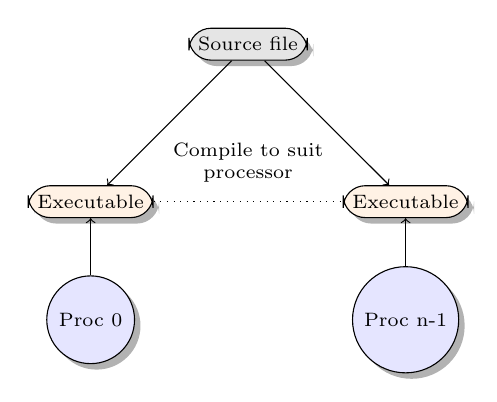
\begin{tikzpicture}
      \node[rectangle, rounded corners=8pt, draw,fill=black!10, drop shadow={fill=black!30,opacity=1}] (S) at (0,2) {\scriptsize  Source file};
      \node[rectangle, rounded corners=8pt, draw,fill=orange!10, drop shadow={fill=black!30,opacity=1}] (E1) at (-2,0) {\scriptsize Executable};
      \node[rectangle, rounded corners=8pt, draw,fill=orange!10, drop shadow={fill=black!30,opacity=1}] (En) at (+2,0) {\scriptsize Executable};
      \node[circle, draw,fill=blue!10, drop shadow={fill=black!30,opacity=1}] (N1) at (-2,-1.5) {\scriptsize Proc 0};
      \node[circle, draw,fill=blue!10, drop shadow={fill=black!30,opacity=1}] (Nn) at (+2,-1.5) {\scriptsize Proc n-1};
      \node at (0,0.5) {\begin{minipage}{2cm}\scriptsize\centering Compile to suit processor\end{minipage}};
      \draw[dotted] (E1) -- (En);
      \draw[->] (S) -- (E1);
      \draw[->] (S) -- (En);
      \draw[->] (N1) -- (E1);
      \draw[->] (Nn) -- (En);
    \end{tikzpicture}
  \end{figure}
\end{columns}
\end{frame}

\begin{frame}
\frametitle{MPMD : Multiple Program Multiple Data model}

In this case, 
\textcolor{blue}{\sl separate programs are executed for several groups of processors}.

Several strategies possible : 
\begin{itemize}
\item \textcolor{blue}{master--slave} : a single
  processor executes a master process and the other processes are started
  from within the master process.

  \begin{minipage}{40mm}
    Basic features :
    \begin{itemize}
    \item Usually \textcolor{blue}{dynamic}
      process creation
    \item Possible only with MPI version 2 .
    \end{itemize}
  \end{minipage}
  \begin{minipage}{55mm}
    \begin{figure}
      \centering
      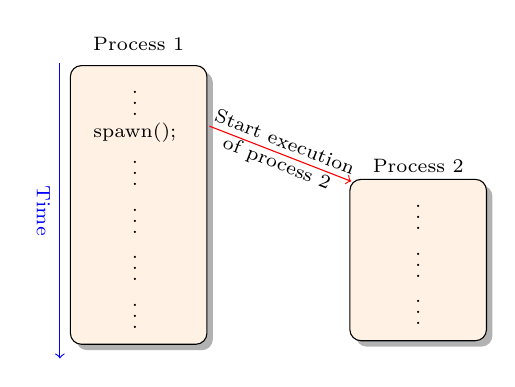
\begin{tikzpicture}
%\draw[step=1mm,color=black!10] (-1,0) grid (5cm,55mm);
%\draw[step=1cm,color=black!50] (-1,0) grid (5cm,55mm);
        \node at (0,4.75) {\scriptsize Process 1};
        \node[rectangle, rounded corners=4pt, draw,fill=orange!10, drop shadow={fill=black!30,opacity=1}] (M) at (0,2.7) 
        {\begin{minipage}{15mm}\scriptsize $\begin{array}{c}
              \vdots \\ \mbox{spawn();} \\ \vdots
              \\ \vdots \\ \vdots \\ \vdots
            \end{array}$\end{minipage}};  
        \node at (3.55,3.2) {\scriptsize Process 2};
        \node[rectangle, rounded corners=4pt, draw,fill=orange!10, drop shadow={fill=black!30,opacity=1}] (S) at (3.55,2) 
        {\begin{minipage}{15mm}\scriptsize\centering $\begin{array}{c}
              \vdots \\ \vdots \\ \vdots
            \end{array}$\end{minipage}};  
        \draw[->,color=blue] (-1,4.5) to node[below,sloped] (y) {\scriptsize Time}(-1,0.75);
        \draw[->,color=red] (0.9,3.7) to node[midway, sloped] (x) 
        {\begin{minipage}{20mm}\scriptsize\centering\color{black}Start execution of process 2\end{minipage}} (2.7,3);
      \end{tikzpicture}
    \end{figure}
  \end{minipage}
\item \textcolor{blue}{Concurrent system} : All programs are independant. Some synchronizations
  are required from time to time. Option available with all MPI versions.
\end{itemize}
\end{frame}

\begin{frame}{Identification of a processus}

To manage a part of data or for control statements, an id must be affected for each process.
Ever more, to split data accordingly, the number of processes launched for the application must be known.

\textbf{Example} : let's consider a parallel sum of two vectors of length \textsl{n}. Each process must sum the same amount of data
than other processes (for load balancing).
\begin{itemize}
\item Amount of data to sum in each vector for a process ? Retrieve the number of processes nbProcs executing our code.
Number of elements in each vector to sum : $n_{l} = \frac{n}{\mathrm{nbProcs}}$.
\item Which elements in each vector a process must sum ? Each process has an unique identifiant $r$ : $0\leq r < \mathrm{nbProcs}$.
For process $r$ : caring about coefficients with indices $i$ as $n_{l}r \leq i < (n_{l}+1)r$ : we done a \textbf{partition} of the
data of each vector.
\end{itemize}

\end{frame}

\begin{frame}
\frametitle{Basic send and receive routines}

Passing datas between processes using \texttt{send()} and
\texttt{recv()} library calls to send/receive a message.

\begin{figure}
  \centering
  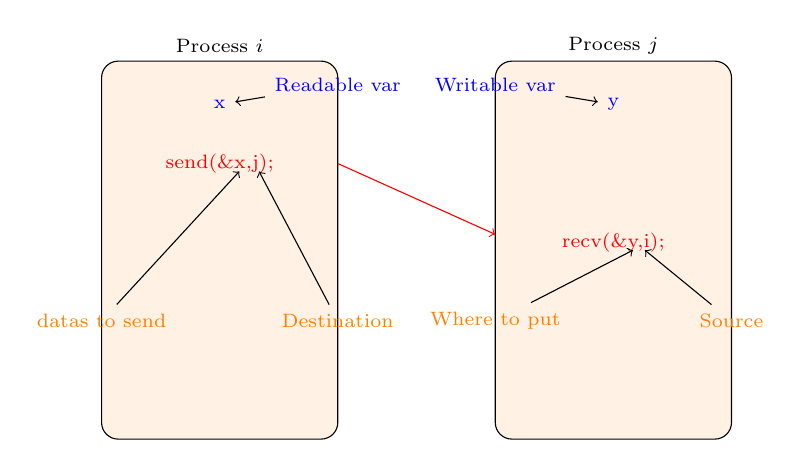
\begin{tikzpicture}
    %\draw[step=1mm,color=black!10] (0,0) grid (10cm,55mm);
    %\draw[step=1cm,color=black!50] (0,0) grid (10cm,55mm);
    \node at (1.5,5) {\scriptsize Process $i$};
    \node at (6.5,5) {\scriptsize Process $j$};
    \draw[rounded corners=6pt,draw,fill=orange!10] (0,4.8) rectangle (3,0);
    \draw[rounded corners=6pt,draw,fill=orange!10] (5,4.8) rectangle (8,0);
    \node[color=blue] at (1.5,4.25) (x) {\scriptsize x};
    \node[color=blue] at (6.5,4.25) (y) {\scriptsize y};
    \node[color=red] at (1.5,3.5) {\scriptsize send(\&x,j);};
    \node[color=red] at (6.5,2.5) {\scriptsize recv(\&y,i);};
    \node[color=blue] at (3,4.5) (rv) {\scriptsize \textrm{Readable var}};
    \node[color=blue] at (5,4.5) (wv) {\scriptsize \textrm{Writable var}};
    \node[color=orange] at (0,1.5) (wts) {\scriptsize \textrm{datas to send}};
    \node[color=orange] at (3,1.5) (dest) {\scriptsize \textrm{Destination}};
    \node[color=orange] at (5,1.5) (wtp) {\scriptsize \textrm{Where to put}};
    \node[color=orange] at (8,1.5) (src) {\scriptsize \textrm{Source}};
    \draw[->,draw] (rv) --  (x);
    \draw[->,draw] (wv) --  (y);
    \draw[->,draw] (wts) --  (1.75,3.4);
    \draw[->,draw] (wtp) --  (6.75,2.4);
    \draw[->,draw] (dest) --  (2,3.4);
    \draw[->,draw] (src) --  (6.9,2.4);
    \draw[->,color=red] (3,3.5) -- (5,2.6);
  \end{tikzpicture}
\end{figure}
\end{frame}

\begin{frame}
\frametitle{Synchronous message--passing}
\begin{itemize}
\item \alert{Synchronous message--passing routines} \textcolor{blue}{return}
  when the message transfer has been completed;
\item There is no need for message buffer storage.
  \begin{itemize}
  \item The synchronous send routine could wait until complete message
    can be accepted by the receiving process before sending the message;
  \item The synchronous receive routine wait until the message it is excepting arrives.
  \end{itemize}
\item Synchronous routines perform two basic actions : They
  \begin{itemize}
  \item \textcolor{blue}{transfer data} and
  \item \textcolor{blue}{synchronize} processes.
  \end{itemize}
\end{itemize}
\end{frame}

\begin{frame}
\frametitle{\ldots Synchronous message--passing}

A three--way protocol is actually used here :
\begin{itemize}
\item \textbf{Case 1} : \texttt{Process 1} arrives to \texttt{send()} before
  \texttt{Process 2} arrives to \texttt{recv()} :
  \begin{figure}
    \centering
  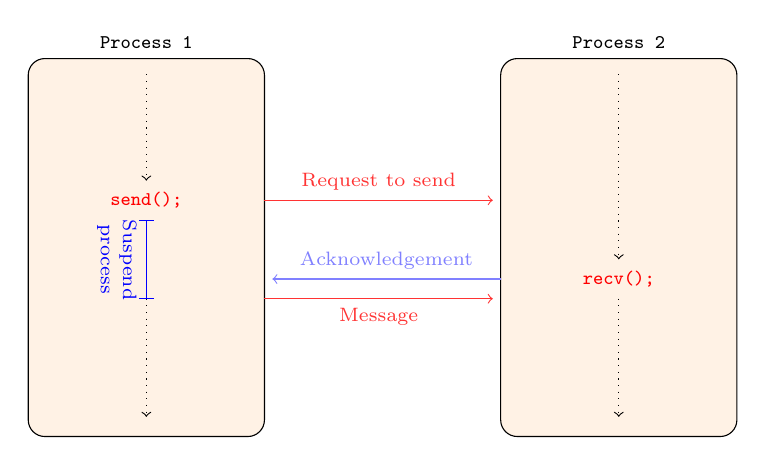
\begin{tikzpicture}
    \node at (1.5,5) {\scriptsize \texttt{Process 1}};
    \node at (7.5,5) {\scriptsize \texttt{Process 2}};
    \draw[rounded corners=6pt,draw,fill=orange!10] (0,4.8) rectangle (3,0);
    \draw[rounded corners=6pt,draw,fill=orange!10] (6,4.8) rectangle (9,0);
    \draw[->,dotted] (1.5,4.6) -- (1.5,3.25);
    \node[color=red] at (1.5,3.0) {\scriptsize \texttt{send();}};
    \draw[->,dotted] (7.5,4.6) -- (7.5,2.25);
    \node[color=red] at (7.5,2) {\scriptsize \texttt{recv();}};
    \draw[|-|,color=blue] (1.5,2.75) to node[below,sloped] (stall)  {\begin{minipage}{1cm}\scriptsize\centering Suspend process\end{minipage}} (1.5,1.75);
    \draw[->,dotted] (1.5,1.75) -- (1.5,0.25);
    \draw[->,dotted] (7.5,1.75) -- (7.5,0.25);
    \draw[->,color=red!80] (3,3) to node[above] (rq) {\scriptsize Request to send} (5.9,3);
    \draw[<-,color=blue!50] (3.1,2) to node[above] (ack) {\scriptsize Acknowledgement} (6,2);
    \draw[->,color=red!80] (3,1.75) to node[below] (msg) {\scriptsize Message} (5.9,1.75);
  \end{tikzpicture}    
  \end{figure}
\end{itemize}
\end{frame}

\begin{frame}
\frametitle{\ldots Synchronous message--passing}
\begin{itemize}
\item \textbf{Case 2} : \texttt{Process 1} arrives to \texttt{send()} after
  \texttt{Process 2} arrives to \texttt{recv()} :
  \begin{figure}
    \centering
  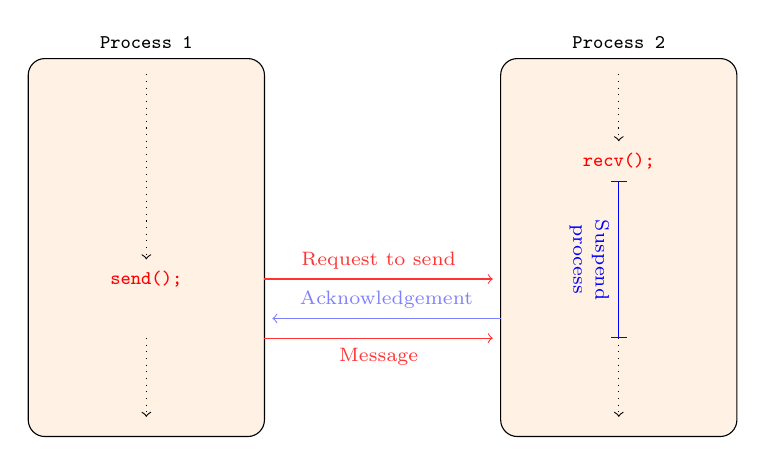
\begin{tikzpicture}
    \node at (1.5,5) {\scriptsize \texttt{Process 1}};
    \node at (7.5,5) {\scriptsize \texttt{Process 2}};
    \draw[rounded corners=6pt,draw,fill=orange!10] (0,4.8) rectangle (3,0);
    \draw[rounded corners=6pt,draw,fill=orange!10] (6,4.8) rectangle (9,0);
    \draw[->,dotted] (1.5,4.6) -- (1.5,2.25);
    \node[color=red] at (1.5,2.0) {\scriptsize \texttt{send();}};
    \draw[->,dotted] (7.5,4.6) -- (7.5,3.75);
    \node[color=red] at (7.5,3.5) {\scriptsize \texttt{recv();}};
    \draw[|-|,color=blue] (7.5,3.25) to node[below,sloped] (stall)  {\begin{minipage}{1cm}\scriptsize\centering Suspend process\end{minipage}} (7.5,1.25);
    \draw[->,dotted] (1.5,1.25) -- (1.5,0.25);
    \draw[->,dotted] (7.5,1.25) -- (7.5,0.25);
    \draw[->,color=red!80] (3,2) to node[above] (rq) {\scriptsize Request to send} (5.9,2);
    \draw[<-,color=blue!50] (3.1,1.5) to node[above] (ack) {\scriptsize Acknowledgement} (6,1.5);
    \draw[->,color=red!80] (3,1.25) to node[below] (msg) {\scriptsize Message} (5.9,1.25);
  \end{tikzpicture}    
  \end{figure}
\end{itemize}
\end{frame}

\begin{frame}
\frametitle{Deadlock}

A tricky problem in synchronous message--passing is the \alert{deadlock} :
it may occur when \textit{\textcolor{blue}{messages cannot be sended because
they are blocked by other messages waiting to be sended and these packets
are blocked in a similar way such that actually} \alert{none of the messages can be send}}.

\underline{Example} : 
\begin{itemize}
\item Node 1 wishes to send to 2;
\item Node 2 wishes to send to 3;
\item Node 3 wishes to send to 1;
\end{itemize}
A famous example was introduced by Dijkstra : \alert{5 philosophers}
may think or eat spaghetti using a circular table with 5 plates and 5 forks when hungry.
Eating spaghetti requires two forks (!?). 
A philosopher release his forks when he is no more hungry.
A deadlock appears when all philosophers are present and all held the right--hand side fork.
\end{frame}

\begin{frame}
\frametitle{Blocking and nonblocking message--passing}

\alert{Blocking}
\begin{itemize}
\item This term is used to describe routines that \textcolor{blue}{do not return} until the transfer is \textcolor{blue}{completed}.
\item More precisely, the routines are \textcolor{blue}{blocked from continuing} the process code;
\item Generally speaking, the terms \alert{synchronous} and \alert{blocking}
  are synonymous.
\end{itemize}

\alert{Non--blocking}
\begin{itemize}
\item This term is used to describe routines that \textcolor{blue}{return whether or not the message had been received}
\end{itemize}

\textsl{\textcolor{brown}{Warning}} : The general terms were redefined in MPI, see below...
\end{frame}

\begin{frame}
\frametitle{MPI definition of blocking and nonblocking}

\alert{blocking} -- Return after their local actions are finished, though the
message transfer may not have been completed (E.g., for \texttt{send()} it
may return after the data are put in buffer to be send ).

\alert{Nonblocking} -- Return immediately. In such a case, it is assumes that
the \textcolor{blue}{data storage} to be used for the transfer \textcolor{blue}{is not modified} by the subsequent statements before the transfer is completed and it us the programmer duty to ensure this.

\textsl{\textcolor{brown}{Notice} : This type of message is based on the use of
\textcolor{blue}{message buffers} between the source and destination processes. As the buffers are of finite length, it may happend that the \texttt{send()} routine is blocked because the available buffer space has been exhausted.}
\end{frame}

\begin{frame}
\frametitle{Message tag}

A \alert{message tag} is an extra information put in the message to 
differentiate between different messages being sent.

Example :

\begin{center}
\begin{tabular}{c|c}
$\vdots$ & $\vdots$ \\
\texttt{send(\&x,2,\textcolor{red}{5});} & \texttt{recv(\&x,1,\textcolor{red}{5});} \\
$\vdots$ & $\vdots$ \\ \hline
( Process 1 ) & ( Process 2 )
\end{tabular}
\end{center}

The tag 5 is used to match the send statement in \texttt{process 1} to the receive statement in \texttt{process 2}.

\underline{Notice} : If such a special type matching is not required, then a
\alert{wild card} message tag is used, so that \texttt{recv()} will match
\textcolor{blue}{any} \texttt{send()}.
\end{frame}

\begin{frame}
\frametitle{Broadcast}

\alert{Broadcast} is used to send the same message \textcolor{blue}{to all}
processes concerned with the problem

\alert{Multicast} is similar, but it is used to send a message
\textcolor{blue}{to a defined group} of processes.
\begin{figure}
  \centering
  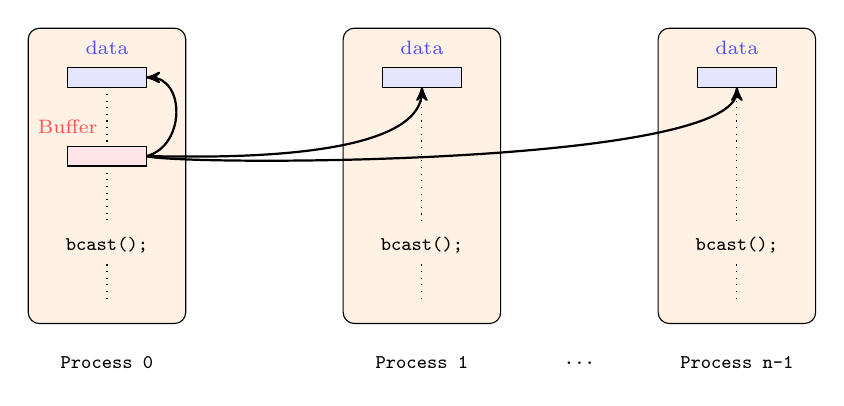
\begin{tikzpicture}
    \node at (1,0) {\scriptsize \texttt{Process 0}};
    \node at (5,0) {\scriptsize \texttt{Process 1}};
    \node at (9,0) {\scriptsize \texttt{Process n-1}};
    \node at (7,0) {\scriptsize \texttt{\ldots}};
    \draw[rounded corners=4pt,draw,fill=orange!10] (0,0.5) rectangle (2,4.25);
    \draw[rounded corners=4pt,draw,fill=orange!10] (4,0.5) rectangle (6,4.25);
    \draw[rounded corners=4pt,draw,fill=orange!10] (8,0.5) rectangle (10,4.25);
    \draw[fill=blue!10,draw] (0.5,3.5) rectangle (1.5,3.75);
    \node[color=blue!70] at (1,4) {\scriptsize data};
    \draw[fill=blue!10,draw] (4.5,3.5) rectangle (5.5,3.75);
    \node[color=blue!70] at (5,4) {\scriptsize data};
    \draw[fill=blue!10,draw] (8.5,3.5) rectangle (9.5,3.75);
    \node[color=blue!70] at (9,4) {\scriptsize data};
    \draw[fill=red!10,draw] (0.5,2.5) rectangle (1.5,2.75);
    \node[color=red!70] at (0.5,3) {\scriptsize Buffer};
    \draw[dotted] (1,3.5) -- (1,2.75);
    \draw[dotted] (1,2.5) -- (1,1.75);
    \node at (1,1.5) {\scriptsize \texttt{bcast();}};
    \draw[dotted] (5,3.5) -- (5,1.75);
    \node at (5,1.5) {\scriptsize \texttt{bcast();}};
    \draw[dotted] (9,3.5) -- (9,1.75);
    \node at (9,1.5) {\scriptsize \texttt{bcast();}};
    \draw[-stealth',thick] (1.5,2.625) .. controls (2,2.75) and (2,3.625) .. (1.5,3.625);
    \draw[-stealth',thick] (1.5,2.625) .. controls (2,2.625) and (5,2.5) .. (5,3.5);
    \draw[-stealth',thick] (1.5,2.625) .. controls (2,2.5) and (9,2.5) .. (9,3.5);
    \draw[dotted] (1,1.25) -- (1,0.75);
    \draw[dotted] (5,1.25) -- (5,0.75);
    \draw[dotted] (9,1.25) -- (9,0.75);
  \end{tikzpicture}    
\end{figure}
\end{frame}

\begin{frame}
\frametitle{Scatter}

\alert{Scatter} is used to send \textcolor{blue}{each element in an array} of data of the
sending process to corresponding separate processes ( datum from the
$i^{th}$ location goes to the $i^{th}$ process ).

\begin{figure}
  \centering
  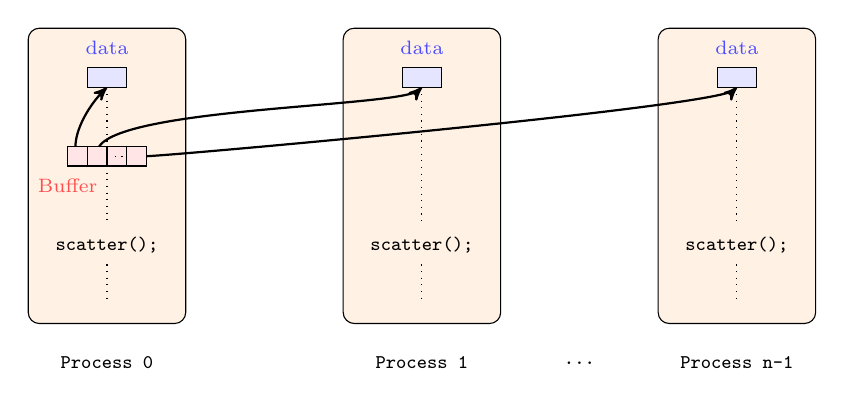
\begin{tikzpicture}
    % \draw[step=1mm,color=black!10] (0,0) grid (3cm,3cm);
    % \draw[step=1cm,color=black!50] (0,0) grid (3cm,3cm);

    \node at (1,0) {\scriptsize \texttt{Process 0}};
    \node at (5,0) {\scriptsize \texttt{Process 1}};
    \node at (9,0) {\scriptsize \texttt{Process n-1}};
    \node at (7,0) {\scriptsize \texttt{\ldots}};
    \draw[rounded corners=4pt,draw,fill=orange!10] (0,0.5) rectangle (2,4.25);
    \draw[rounded corners=4pt,draw,fill=orange!10] (4,0.5) rectangle (6,4.25);
    \draw[rounded corners=4pt,draw,fill=orange!10] (8,0.5) rectangle (10,4.25);
    \draw[fill=blue!10,draw] (0.75,3.5) rectangle (1.25,3.75);
    \node[color=blue!70] at (1,4) {\scriptsize data};
    \draw[fill=blue!10,draw] (4.75,3.5) rectangle (5.25,3.75);
    \node[color=blue!70] at (5,4) {\scriptsize data};
    \draw[fill=blue!10,draw] (8.75,3.5) rectangle (9.25,3.75);
    \node[color=blue!70] at (9,4) {\scriptsize data};
    \draw[fill=red!10,draw, step=0.25] (0.5,2.5) rectangle (1.5,2.75);
    \draw[draw, step=0.25] (0.49,2.49) grid (1.5,2.75);
    \draw[dotted] (1.1,2.625) -- (1.24,2.625);
    \node[color=red!70] at (0.5,2.25) {\scriptsize Buffer};
    \draw[dotted] (1,3.5) -- (1,2.75);
    \draw[dotted] (1,2.5) -- (1,1.75);
    \node at (1,1.5) {\scriptsize \texttt{scatter();}};
    \draw[dotted] (5,3.5) -- (5,1.75);
    \node at (5,1.5) {\scriptsize \texttt{scatter();}};
    \draw[dotted] (9,3.5) -- (9,1.75);
    \node at (9,1.5) {\scriptsize \texttt{scatter();}};
    \draw[-stealth',thick] (0.6,2.75) .. controls (0.6,2.95) and (0.75,3.25) .. (1,3.5);
    \draw[-stealth',thick] (0.9,2.75) .. controls (1.25,3.25) and (4.75,3.25) .. (5,3.5);
    \draw[-stealth',thick] (1.5,2.625) .. controls (1.75,2.625) and (8.75,3.25) .. (9,3.5);
    \draw[dotted] (1,1.25) -- (1,0.75);
    \draw[dotted] (5,1.25) -- (5,0.75);
    \draw[dotted] (9,1.25) -- (9,0.75);
  \end{tikzpicture}    
\end{figure}

\end{frame}

\begin{frame}
\frametitle{gather}

\alert{Gather} is the opposite operation : the receiving process \alert{collect}
\textcolor{blue}{in an array} the data sent by separate processes ( datum from the
$i^{th}$ process goes to the $i^{th}$ location ).

\begin{figure}
  \centering
  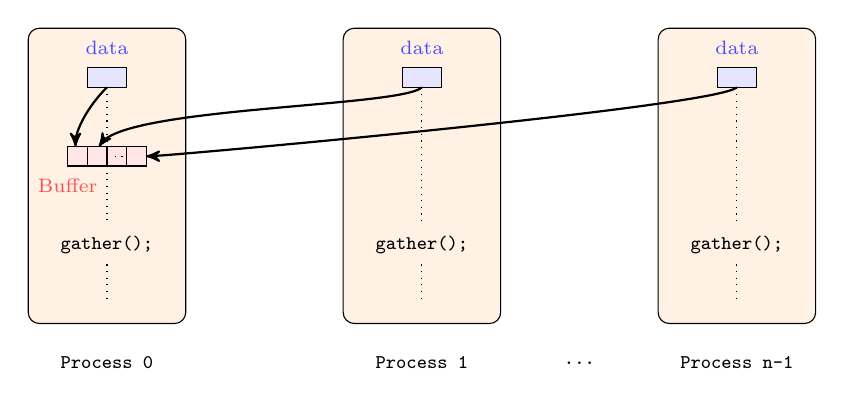
\begin{tikzpicture}
    % \draw[step=1mm,color=black!10] (0,0) grid (3cm,3cm);
    % \draw[step=1cm,color=black!50] (0,0) grid (3cm,3cm);
    \node at (1,0) {\scriptsize \texttt{Process 0}};
    \node at (5,0) {\scriptsize \texttt{Process 1}};
    \node at (9,0) {\scriptsize \texttt{Process n-1}};
    \node at (7,0) {\scriptsize \texttt{\ldots}};
    \draw[rounded corners=4pt,draw,fill=orange!10] (0,0.5) rectangle (2,4.25);
    \draw[rounded corners=4pt,draw,fill=orange!10] (4,0.5) rectangle (6,4.25);
    \draw[rounded corners=4pt,draw,fill=orange!10] (8,0.5) rectangle (10,4.25);
    \draw[fill=blue!10,draw] (0.75,3.5) rectangle (1.25,3.75);
    \node[color=blue!70] at (1,4) {\scriptsize data};
    \draw[fill=blue!10,draw] (4.75,3.5) rectangle (5.25,3.75);
    \node[color=blue!70] at (5,4) {\scriptsize data};
    \draw[fill=blue!10,draw] (8.75,3.5) rectangle (9.25,3.75);
    \node[color=blue!70] at (9,4) {\scriptsize data};
    \draw[fill=red!10,draw, step=0.25] (0.5,2.5) rectangle (1.5,2.75);
    \draw[draw, step=0.25] (0.49,2.49) grid (1.5,2.75);
    \draw[dotted] (1.1,2.625) -- (1.24,2.625);
    \node[color=red!70] at (0.5,2.25) {\scriptsize Buffer};
    \draw[dotted] (1,3.5) -- (1,2.75);
    \draw[dotted] (1,2.5) -- (1,1.75);
    \node at (1,1.5) {\scriptsize \texttt{gather();}};
    \draw[dotted] (5,3.5) -- (5,1.75);
    \node at (5,1.5) {\scriptsize \texttt{gather();}};
    \draw[dotted] (9,3.5) -- (9,1.75);
    \node at (9,1.5) {\scriptsize \texttt{gather();}};
    \draw[-stealth',thick] (1,3.5) .. controls (0.75,3.25) and (0.6,2.95) .. (0.6,2.75);
    \draw[-stealth',thick] (5,3.5) .. controls (4.75,3.25) and (1.25,3.25) .. (0.9,2.75);
    \draw[-stealth',thick] (9,3.5) .. controls (8.75,3.25) and (1.75,2.625) .. (1.5,2.625);
    \draw[dotted] (1,1.25) -- (1,0.75);
    \draw[dotted] (5,1.25) -- (5,0.75);
    \draw[dotted] (9,1.25) -- (9,0.75);
  \end{tikzpicture}    
\end{figure}

\end{frame}

\begin{frame}
\frametitle{Reduce}

\alert{Reduce} combines \texttt{gather()} routine with an arithmetic or logical operation :
the receiving process \textcolor{blue}{collects} the data, \textcolor{blue}{applies}
the operation and \textcolor{blue}{saves} it in its own memory.

\begin{figure}
  \centering
  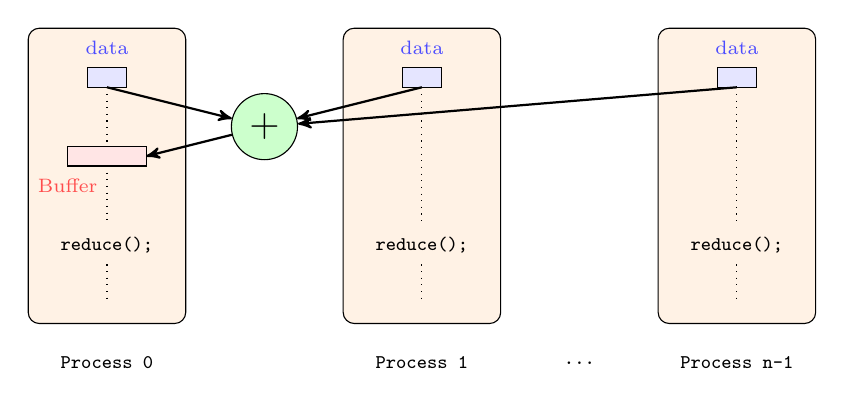
\begin{tikzpicture}
    % \draw[step=1mm,color=black!10] (0,0) grid (3cm,3cm);
    % \draw[step=1cm,color=black!50] (0,0) grid (3cm,3cm);
    \node at (1,0) {\scriptsize \texttt{Process 0}};
    \node at (5,0) {\scriptsize \texttt{Process 1}};
    \node at (9,0) {\scriptsize \texttt{Process n-1}};
    \node at (7,0) {\scriptsize \texttt{\ldots}};
    \draw[rounded corners=4pt,draw,fill=orange!10] (0,0.5) rectangle (2,4.25);
    \draw[rounded corners=4pt,draw,fill=orange!10] (4,0.5) rectangle (6,4.25);
    \draw[rounded corners=4pt,draw,fill=orange!10] (8,0.5) rectangle (10,4.25);
    \draw[fill=blue!10,draw] (0.75,3.5) rectangle (1.25,3.75);
    \node[color=blue!70] at (1,4) {\scriptsize data};
    \draw[fill=blue!10,draw] (4.75,3.5) rectangle (5.25,3.75);
    \node[color=blue!70] at (5,4) {\scriptsize data};
    \draw[fill=blue!10,draw] (8.75,3.5) rectangle (9.25,3.75);
    \node[color=blue!70] at (9,4) {\scriptsize data};
    \draw[fill=red!10,draw, step=0.25] (0.5,2.5) rectangle (1.5,2.75);
    \node[color=red!70] at (0.5,2.25) {\scriptsize Buffer};
    \draw[dotted] (1,3.5) -- (1,2.75);
    \draw[dotted] (1,2.5) -- (1,1.75);
    \node at (1,1.5) {\scriptsize \texttt{reduce();}};
    \draw[dotted] (5,3.5) -- (5,1.75);
    \node at (5,1.5) {\scriptsize \texttt{reduce();}};
    \draw[dotted] (9,3.5) -- (9,1.75);
    \node at (9,1.5) {\scriptsize \texttt{reduce();}};
    \node[shape=circle,fill=green!20,draw] (plus) at (3,3) {\Large +};
    \draw[-stealth',thick] (1,3.5) to (plus);
    \draw[-stealth',thick] (5,3.5) to (plus);
    \draw[-stealth',thick] (9,3.5) to (plus);
    \draw[-stealth',thick] (plus) to (1.5,2.625);
    \draw[dotted] (1,1.25) -- (1,0.75);
    \draw[dotted] (5,1.25) -- (5,0.75);
    \draw[dotted] (9,1.25) -- (9,0.75);
  \end{tikzpicture}    
\end{figure}

\end{frame}

\section{Software tools}

\subsection{PVM}
\begin{frame}
\frametitle{Software tools}
\alert{PVM (Parallel Virtual Machine)}
\begin{itemize}
\item A first wildly accepted attempt to use a workstation cluster as a multicomputer.
\item It may be used to run programs on both homogeneous or heterogeneous multicomputers.
\item It has a collection of library routines to be used with C or FORTRAN programs.
\item It's free.
\end{itemize}
\end{frame}

\subsection{MPI}
\begin{frame}
\frametitle{\ldots Software tools}

\alert{MPI (Message Passing Interface)}
\begin{itemize}
\item It is a standard developed by a group of academies and industrial people
  to increase the use and the portability of message passing.
\item Several free implementation exists
\item It has a collection of library routines to be used with C, C++ and Fortran
programs. Some interface exist to use MPI with Python programs.
\item It may be used to run programs on both homogeneous or heterogeneous multicomputers.
\end{itemize}
\end{frame}

\begin{frame}
\frametitle{MPI}

\textcolor{orange!75}{General} : MPI is a \textcolor{blue}{standard} with various
implementation

\textcolor{orange!75}{Process creation and execution} : Defined at the running
of the programs. The \textcolor{blue}{set of computers} used for the
problem can be defined prior the running of the programs ( A convenient
way to do this is by using a \alert{machinefile} listing the names
of the computers available. This machinefile is then read by MPI.

\textcolor{orange!75}{Communications} : One defines the \alert{scope} of the
communication operation; the set of all involved processes may be
accessed using the predefined variable \texttt{\textcolor{orange}
{MPI\_COMM\_WORLD}}; each process has an unique rank, a number
from 0 to $n-1$ ( where $n$ is the number of processes ); other
communication groups may be defined.

\end{frame}

\begin{frame}[fragile]
\frametitle{\ldots MPI}

\begin{block}{Shape of an MPI program}
\begin{lstlisting}
int main(int argc, char *argv[])
{
  int myrank, nbprocs;
  MPI_Init(&argc, &argv);  /* Initialize MPI context */
  /* Find the rank of the process */
  MPI_Comm_rank(MPI_COMM_WORLD, &myrank);
  /* Find the number of processes running the program */
  MPI_Comm_size(MPI_COMM_WORLD, &nbprocs);
  ...
  if (myrank == 0)
  {
     /* Do something if first processor */
  }
  else
  {
     /* Do something different for others processors */
  }
  MPI_Finalize();/*Delete MPI context */
}
\end{lstlisting}
\end{block}
\end{frame}

\begin{frame}
\frametitle{\ldots MPI}
\textcolor{orange}{Point--to--point communication} : Message tags
and wild cards may be used ( \texttt{MPI\_ANY\_TAG} or
\texttt{MPI\_ANY\_SOURCE} )\\[5mm]

\textcolor{orange}{Blocking routines} : Return when they are
locally complete, i.e, when the location used for the message
can be used again without affecting the message being sent;
general format :

{\scriptsize
\begin{tabular}{ll}
\texttt{\textcolor{red}{MPI\_Send}(}& \texttt{void* buf, int count, MPI\_Datatype datatype,}\\
                                  & \texttt{int dest, int tag, MPI\_Comm comm)}
\end{tabular}
where \texttt{buf}--address of send buffer, 
      \texttt{count}--number of items to send,
      \texttt{datatype}--Data type of each item,
      \texttt{dest}--Rank of destination process,
      \texttt{tag}--Message tag,
      \texttt{comm}--Communicator\\
\begin{tabular}{ll}
\texttt{\textcolor{red}{MPI\_Recv}(}& \texttt{void* buf, int count, MPI\_Datatype datatype,}\\
                                  & \texttt{int source, int tag, MPI\_Comm comm, MPI\_Status *status)}
\end{tabular}
where \texttt{buf}--address of receive buffer, 
      \texttt{count}--Maximum number of items to receive,
      \texttt{datatype}--Data type of each item,
      \texttt{dest}--Rank of source process,
      \texttt{tag}--Message tag,
      \texttt{comm}--Communicator,
      \texttt{status} -- Status after operation
}

\end{frame}

\begin{frame}[fragile]
\frametitle{\ldots MPI}

\textcolor{orange}{Example ( Blocking communication )} : To send
an integer \texttt{x} from process 0 to process 1 :

\begin{lstlisting}
MPI_Comm_rank(MPI_COMM_WORLD,&myrank);
if (myrank == 0){
  int x;
  MPI_Send(&x, 1, MPI_INT, 1, 73, MPI_COMM_WORLD);
  } else if (myrank == 1){
  int x;
  MPI_Status status;
  MPI_Recv(&x,1,MPI_INT, 0,73, MPI_COMM_WORLD,&status);
  }
\end{lstlisting}
\end{frame}

\begin{frame}[fragile]
\frametitle{\ldots MPI}
\small
\textcolor{orange}{Non--blocking communication} : \texttt{MPI\_Isend()}
and \texttt{MPI\_Irecv()} -- return ``immediately'', even if the
communication is not safe; to be used in combination with
\texttt{MPI\_Wait()} and \texttt{MPI\_Test()} in order to ensure
a complete communication.

\textcolor{orange}{Example (non--blocking communication)} -- same example

\begin{lstlisting}
MPI_Status status;
int x;
if (myrank == 0){
  MPI_Request req1;
  MPI_ISend(&x, 1, MPI_INT, 1, 73, MPI_COMM_WORLD,&req1);
  compute();
  MPI_Wait(&req1, &status);
  } else if (myrank == 1){
  MPI_Recv(&x,1,MPI_INT, 0,73, MPI_COMM_WORLD,&status);
  }
\end{lstlisting}

\end{frame}

\begin{frame}
\frametitle{\ldots MPI}

\textcolor{orange}{Send communication modes} : Four basic modes are
\begin{enumerate}
\item \alert{Standard mode send} -- It is not assumed that the
corresponding receive routine has started (buffer space is not
defined here; if buffering is provided, send can be complete
before the corresponding receive was reached )
\item \alert{Buffered mode} -- Send may start and return before
a matching receive was reached ( here it is necessary to specify
buffer space )
\item \alert{Synchronous mode} -- Send and receive have to complete
together (however, they may start at any time )
\item \alert{Ready mode} -- Send can only start if a matching
receive was already reached (use it with care... )
\end{enumerate}
\end{frame}

\begin{frame}
\frametitle{\ldots MPI}

\textcolor{orange}{Collective communication} : This applies to
processes included in a communicator. The main operations are :
\begin{itemize}
\item \alert{\texttt{MPI\_Bcast()}}-- Broadcast from root to all other processes
\item \alert{\texttt{MPI\_Gather()}} -- Gather values from processes in the group
\item \alert{\texttt{MPI\_Scatter()}} -- Scatter parts of the buffer to processes
\item \alert{\texttt{MPI\_Reduce()}} -- Collect and combine values from processes
\item \alert{\texttt{MPI\_Allreduce()}} -- Combine reduce and broadcast
\end{itemize}

\textcolor{orange}{Barrier} : May be used to synchronize processes
by stopping each process until all have reached the barrier call
\begin{itemize}
\item \alert{\texttt{MPI\_Barrier(MPI\_Comm comm)}}
\end{itemize}
\end{frame}

\begin{frame}
\frametitle{Example of MPI program}

We illustrate MPI programming style with a simple question :
\textcolor{blue}{\rm add the numbers from a file using multiple
processes}

A master--slave approach is used :
\begin{itemize}
\item A master process ( process 0 ) detects the number of processes
from communicator, reads data from the file and sends them to
all processes ( by broadcast ).
\item Each process ( including the master ) identifies its portion
of data and adds them.
\item The master collects the partial sums and adds them
(using \texttt{reduce} statements ) and prints the final result.
\end{itemize}
\end{frame}

\begin{frame}[fragile]
\frametitle{MPI program}
\begin{lstlisting}
# include <mpi.h>
# include <stdio.h>
# include <math.h>
# define MAXSIZE 1000
void main(int argc, char *argv) {
  int myid, numprocs;
  int data[MAXSIZE], i, x, low, high, myresult, result;
  char fn[255];
  char *fp;
  MPI_Init(&argc, &argv);
  MPI_Comm_size(MPI_COMM_WORLD,&numprocs);
  MPI_Comm_rank(MPI_COMM_WORLD,&myid);
  if ( myid == 0 ) {
    if ( (fp = fopen("rand_data.txt", "r")) == NULL ) {
      printf("Can't open the input file\n");
      MPI_Abort(MPI_COMM_WORLD,1);
    }    
\end{lstlisting}
\end{frame}

\begin{frame}[fragile]
\frametitle{\ldots MPI program}
\begin{lstlisting}
    for (i=0; i<MAXSIZE; i++) fscanf(fp,"%d",&data[i]);
  }
  /* Broadcast data */
  MPI_Bcast(data,MAXSIZE,MPI_INT,0,MPI_COMM_WORLD);
  /* Add my portion of data */
  x = MAXSIZE/numprocs;
  low  = myid*x;
  high = low + x;
  myresult = 0;
  for ( i = low; i < high; i++ )
    myresult += data[i];
  printf("I got %d from %d\n",myresult,myid);
  /*Compute global sum */
  MPI_Reduce(&myresult, &result, 1, MPI_INT, MPI_SUM, 0, 
             MPI_COMM_WORLD);
  if (myid == 0) printf("The sum is %d.\n",result);
  MPI_Finalize();
}
\end{lstlisting}
\end{frame}
\section{Parallel program evaluation}
\begin{frame}
\frametitle{Parallel program evaluation}

\alert{Program evaluation} :
\begin{itemize}
\item Both \textcolor{royalblue}{theorical} and
  \textcolor{royalblue}{empirical} techniques may be used
to determine the efficiency of (parallel) programs.
\item The ultimate goal is to discriminate between various
parallel processing techniques; a fine tune is also necessary
to find the best \alert{number of processes} and a good balance
of the \alert{computation time} and of the \alert{communication
time} of each process.
\item An extra goal to find out if a parallel processing approach
is actually better suited than a ( usually simpler ) sequential one.
\end{itemize}
\end{frame}

\begin{frame}
\frametitle{Parallel execution time}
\small
\alert{Theorical evaluation of parallel programs} is based on :
\begin{itemize}
\item \textcolor{violet}{Parallel execution time}, $t_{p}$,
  consists of the \alert{computation time} $t_{comp}$ and
  the \alert{communication time} $t_{comm}$, namely :
  \[
  t_{p} = t_{comp} + t_{comm}
  \]
\item \textcolor{violet}{Computation time}, $t_{comp}$,
  is estimated similarly as in the case of sequential
   algorithms ( Supposed here that all processes use identical
   computers )
 \item \textcolor{violet}{Communication time}, $t_{comm}$,
   consists of the \alert{startup time} $t_{startup}$
   ( also called ``message latency'' ) and the
   \alert{time to send data} $n.t_{data}$, where
   $t_{data}$ is the time to transfer a data word, namely :
   \[
   t_{comm} = t_{startup} + n.t_{data}
   \]
 \end{itemize}
\end{frame}

\begin{frame}
\frametitle{Latency hiding}

\begin{itemize}
\item A general method to overcome the significant message
  communication time is to \textcolor{royalblue}{overlap
    communication with subsequent computations}
\item \textcolor{royalblue}{Nonblocking send routines}
  are particulary useful to enable latency hiding
\item Another technique is to use \textcolor{royalblue}{multi--threading}
\item Beware updating of sended datas !
\end{itemize}
\end{frame}

\begin{frame}
\frametitle{Cost--optimal algorithms}

A \alert{cost--optimal} ( or \alert{processor--time optimal} )
algorithm is one such that
\begin{center}
{\small
(parallel time complexity)$\times$ (number of procs.)\\
 =
\\
(sequential time complexity)
}
\end{center}
\textcolor{violet}{Example} :
\begin{itemize}
\item Suppose the best know algorithm for problem $P$
  has time complexity $O(n\log n)$
\item A parallel algorithm solving the same problem using $n$ 
processes and having the time complexity $O(\log n)$ is 
cost--optimal, while a parallel algorithm which uses
$n^{2}$ processes and has time complexity
$O(1)$ is not cost-optimal.
\end{itemize}
\end{frame}

\begin{frame}[fragile]
\frametitle{Evaluating programs empirically}

\alert{Measuring execution time} : To measure
the execution time between point $L_{1}$ and
$L_{2}$ in the code, one may use the following construction :
\begin{lstlisting}
L1: double t1 = MPI_Wtime();
    ...
L2: double t2 = MPI_Wtime();
    double ellapsedTime = t2-t1;
    printf("Elapsed time : %5.2g seconds\n",elapsedTime);
\end{lstlisting}
\end{frame}

\begin{frame}[fragile]
\frametitle{\ldots Evaluating programs empirically}
\small
\alert{Communication time by Ping--Pong methods} :
To empirically estimate the communication time
from a process $P_{1}$ to a process $P_{2}$ one may
use the following method : \textcolor{royalblue}{Immediately}
after receiving the message $P_{2}$, 
\textcolor{royalblue}{send the message back} to $P_{1}$.
\begin{lstlisting}
double t1 = MPI_Wtime();
if ( myrank == P1 )
{
  send(&x,P2); recv(&x,P2);
}
else if ( myrank == P2 )
{
  recv(&x,P1); send(&x,P1);
}
double t2 = MPI_Wtime();
elapsedTime = 0.5*(t2-t1);
\end{lstlisting}

\textcolor{violet}{Remark} : Another method is to use
\texttt{MPI\_Barrier} after sending or receiving
\end{frame}

\begin{frame}
\frametitle{Debugging strategy}
An useful \alert{three--step approach} to debugging
message--passing programs is :
\begin{enumerate}
\item If possible, run the program as a single process and debug
  as a normal \textcolor{royalblue}{sequential program}.
\item Execute the program using 
  \textcolor{royalblue}{two to four multi--tasked processes}
  on a \textcolor{royalblue}{single computer}. Now, examine
  actions such as checking that messages are indeed being
  sent to correct places. It is very common to make
  mistakes with message tags and have messages sent to wrong
  places.
\item Execute the program using \textcolor{royalblue}{two
    to four processes} but now across 
  \textcolor{royalblue}{several computers}. This step help to
  find the impact of netword delays on synchronization and timing
  constraints of your program.
\end{enumerate}
\end{frame}
\end{document}